% Chapter 5

\chapter{\uppercase{Results}} % Main chapter title
\label{chap5} % For referencing
To use the program, the user has to first input the headers used. The headers for klee and assert must not be included. The user must also enter the name of the functions (reference and error implementation) and the definition of these functions. The user then has to select the type of argument needed by the functions and any additional constraints on the input.\\
\begin{figure}[h]
\centering
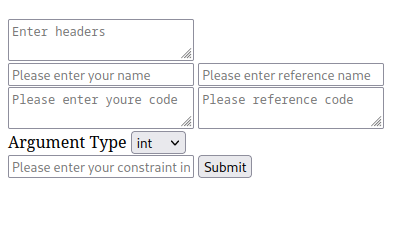
\includegraphics[width=1\textwidth]{5/ui.png}
\caption{User Interface for the program}
\label{fig:ui}
\end{figure}
The program was tested using some programs that are attached in the appendix. These programs were chosen to depict errors that arise from different mistakes in programming. Additional information about these programs are given in the table \ref{tab:my_label}. \\\\

\begin{table}[ ]
    \centering
    \begin{tabularx}{\textwidth} { 
        | >{\raggedright\arraybackslash}X |
        | >{\centering\arraybackslash}X 
        | >{\centering\arraybackslash}X 
        | >{\centering\arraybackslash}X 
        | >{\centering\arraybackslash}X 
        | >{\centering\arraybackslash}X 
        | >{\raggedleft\arraybackslash}X | }
        \hline
        Program & Error Type & LOC (ref) & LOC (err) & Iterative & Recursive & Time \\
        \hline
        isVowel & Incorrect Branch & 34 & 29 & False & False & 1.024  \\
        \hline
        isPrime & Loop Start & 13 & 13 & True & False & 0.903  \\
        \hline
        isPrime & Loop End & 13 & 13 & True & False & 1.089  \\
        \hline
        isPrime & Loop Increment & 13 & 13 & True & False & 0.890  \\
        \hline
        isPrime & Infinite Loop & 13 & 13 & True & False & 46.245  \\
        \hline
        fib & Incorrect Recursion & 10 & 9 & False & True & 0.744  \\
        \hline
    \end{tabularx}
    \caption{Time taken for testing of the C Programs}
    \label{tab:my_label}
\end{table}
The time taken to detect the error was greatest in the case of the infinite loop error type. The other errors were detected in about 1 second when an appropriate constraint was given. The runtime varies depending on various external factors.

The above information is depicted graphically in the chart \ref{fig:runtime}.\\
\begin{figure}[h!]
  \centering
    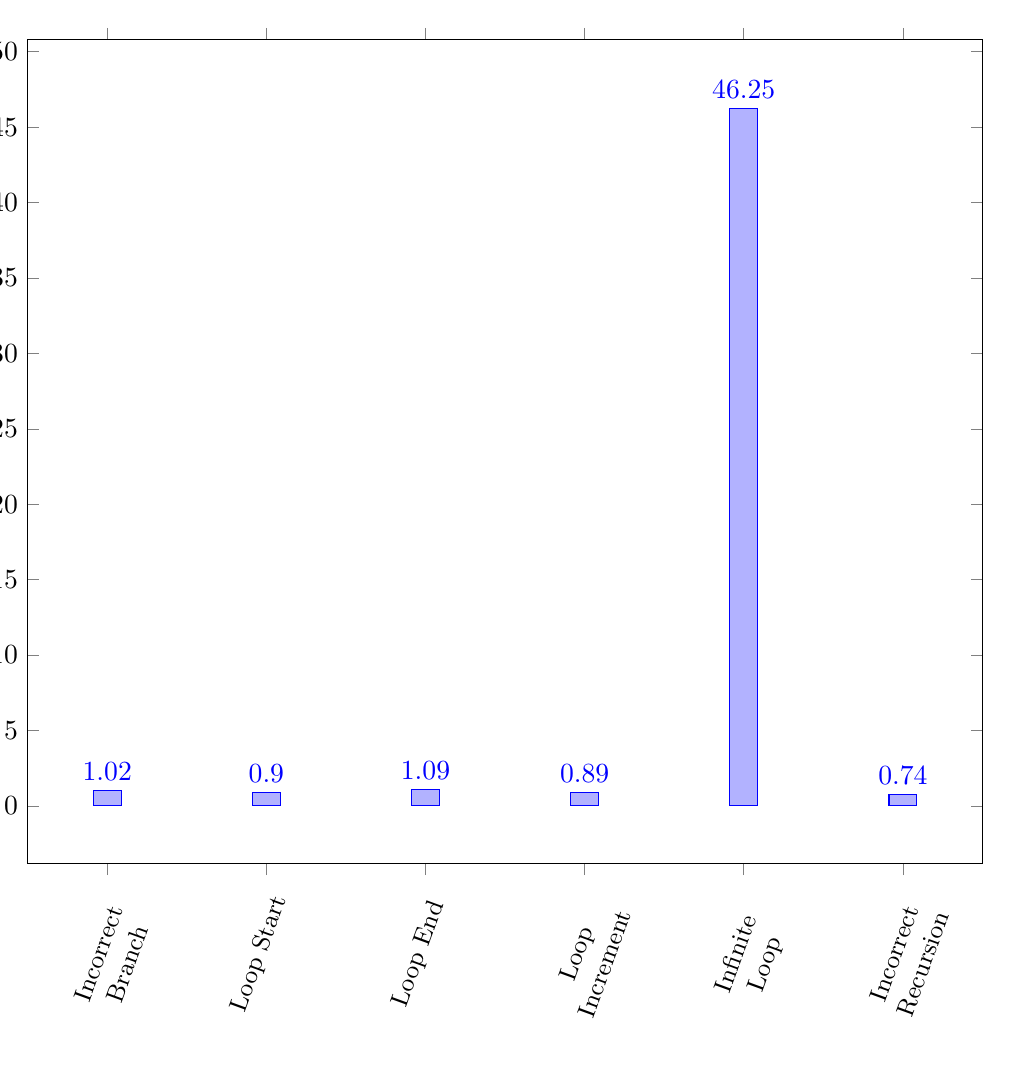
\begin{tikzpicture}[trim axis left]
        \begin{axis}  
        [  
            scale only axis,
            ybar,  
            width=\textwidth,
            ylabel={\ Time in seconds}, % the ylabel must precede a # symbol.  
            x tick label style = {font = \small, text width = 1.7cm, align = center, rotate = 70, anchor = north east},
            symbolic x coords={Incorrect Branch, Loop Start, Loop End, Loop Increment, Infinite Loop, Incorrect Recursion}, % these are the specification of coordinates on the x-axis.  
            xtick=data,  
             nodes near coords, % this command is used to mention the y-axis points on the top of the particular bar.  
            nodes near coords align={vertical},  
            ]  
        \addplot coordinates {(Incorrect Branch,1.024) (Loop Start,0.903) (Loop End,1.089) (Loop Increment,0.890) (Infinite Loop,46.245) (Incorrect Recursion,0.744) };  
        \end{axis}  
    \end{tikzpicture}
  \caption{C statements vs Time taken for execution}
  \label{fig:runtime}
\end{figure}